\section{Evoluzione stellare}

\begin{wordonframe}{da fare: kippenhahn wiegert}
\begin{itemize}
\item main sequence 207'-214' (110-114)
\item Hayashi line 224'-232' (119-123)
\item Stability 234'-246 (124-130)
\item Onset of star formation 248'-255' (131-134)
\item Formation of protostars 256'-265' (135-139)
\item pre-main sequence contraction 266'-270' (140-142)
\item from initial to present sun 271'-276' (142-144)
\item chemical evolution in MS 277'-291' (145-152)
\item He-burning: massive stars 292'-307' (153-160)
\item He-burning:low-mass stars 308'-327' (161-170)
\item Later phases:  328'-343' (171-178)
\item Explosion and collapse 344'-364' (179-189)
\end{itemize}
\end{wordonframe}

\subsection{Pre main sequence ed approccio a ZAMS per stelle di sequenza superiori/inferiori}

\begin{frame}{Traccia di Hayashi}
Primo/secondo core di Larson; Evoluzione di PMS sulla traccia di Hayashi; ruolo di opacit\'a di H- nella verticalit\'a della traccia di Hayashi; fusione deuterio; stelle completamente convettive o con nucleo radiativo. Abbondanza elementi leggeri in stelle di pre-sequenza
\end{frame}

\begin{frame}{Approccio alla ZAMS per stelle di sequenza superiori/inferiori}
dipendenza della ZAMS dall'abbondanza originale di He e metalli; metodo determinazione $DY/DZ$ dal confronto teoria-osservazione per stelle di disco locale parallassate; dipendenza massa minima di transizione dall'abbondanza di He e metalli; influenza sulla ZAMS dell'incertezza degli input fisici e dell'efficienza della convezione
\end{frame}

\subsection{Evoluzione di sequenza principale}

\begin{frame}{Yield of H-burning star analysis}
\begin{itemize}
\item Longest evolutionary phase: larger number of observed stars
\item central/shell-H-burning determine successive phases
\item most important clock is central H-burning termination
\item Final shell H-burning phase in low mass, low-Z star provide distance indicator for old stellar pop
\item count of stars evolving through central H-burning give insight on IMF
\end{itemize}
\end{frame}

\begin{frame}{Major H burning reaction: PP chains}
\begin{columns}[T]\begin{column}{0.5\textwidth}
\begin{align*}
&^1H+^1H\to^2D+\APelectron+\Pnue\\
&^2D+^1H\to^3He+\gamma\\
&T\geq\SI{8e6}{\kelvin}: ^3He+^3He\to^4He+2^1H\tag*{PPI}\\
&T\geq\SI{15e6}{\kelvin}: ^3He+^4He\to^7Be+\gamma\\
&^7Be+\Pelectron\to^7Li+\Pnue\\
&^7Li+^1H\to^4He+^4He\tag*{PPII}\\
&^7Be+^1H\to^8B+\gamma\\
&^8B\to^8Be+\APelectron+\gamma\\
&^8Be\to2^4He
\end{align*}
\end{column}\begin{column}{0.5\textwidth}
\begin{align*}
&r_{pp}=\num{11.5e10}\rho^2X_H^2T_6\expy{-2/3}\exp{-33.81T_6\expy{-1/3}}(1+0.0123T_6\expy{1/3}+0.0109T_6\expy{2/3}+0.00095T_6)\\
&\rho\epsilon(3H\to^3He)=(\SI{6.936}{\mega\ev}-\SI{0.263}{\mega\ev})*\SI{1.602e-6}{\erg}*r_{pp}\\
&\rho\epsilon(^3He(^3He,2p)^4He)=(\SI{6.936}{\mega\ev}-\SI{0.263}{\mega\ev})*\SI{1.602e-6}{\erg}*r_{pp}\\
&\frac{PPI}{PPII+PPIII}=\frac{r_{33}}{r_{34}}=\frac{\lambda_{33}(^3He)^2/2}{\lambda_{34}^3He^4He}
\end{align*}
\end{column}\end{columns}
\end{frame}

\begin{frame}{H burning: CN-NO cycle}
\begin{columns}[T]\begin{column}{0.5\textwidth}
Ciclo CN-NO
\begin{align*}
&^{12}C+^1H\to^{13}N+\gamma\\
&^{13}N\to^{13}C\APelectron+\Pnue\\
&^{13}C+^1H\to^{14}N+\gamma\\
&^{14}N+^1H\to^{15}O+\gamma\\
&^{15}O\to^{15}N+\APelectron+\Pnue\\
&^{15}+^1H\to^{12}+^4He\tag*{CN}\\
&T\geq\SI{20e6}{\kelvin}\tag*{\num{e-4} volte}\\
&^{15}N+^1H\to^{16}O+\gamma\\
&^{16}O+^1H\to^{17}F+\gamma\\
&^{17}F\to^{17}O+\APelectron+\Pnue\\
&^{17}O+^1H\to^{14}N+^4He
\end{align*}
\end{column}\begin{column}{0.5\textwidth}
\begin{align*}
&\epsilon_{CN}(T_6)=\epsilon_{CN}(25)(\frac{T_6}{25})^{16.7}
\end{align*}
\end{column}\end{columns}
\end{frame}

\subsection{Lower main sequence ($M^*\leq1.3\msun{}$)}

\begin{frame}{Da ZAMS a TO for $M^*\leq1.3\msun{}$}
ZAMS: first MS model fully supported by H-burning in which secondary elements are in equilibrium:
\begin{itemize}
\item $^3He$ production in central zones: si forma piccolo core convettivo
\[\TDy{t}{N_3}=N_1N_2\exv{\sigma v}_{12}-2\frac{(N_3)^2}{2}\exv{\sigma v}_{33}-N_3N_4\exv{\sigma v}_{34}\]
\end{itemize}
\begin{columns}[T]\begin{column}{0.4\textwidth}
\begin{figure}[!ht]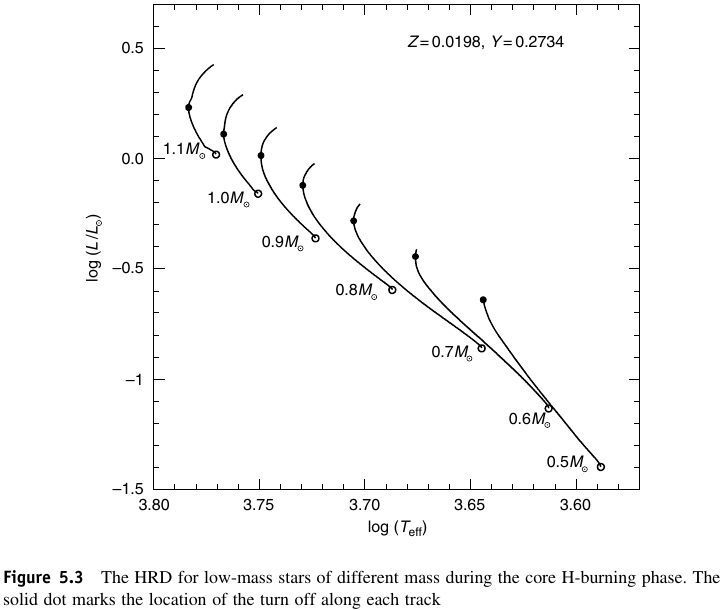
\includegraphics[trim={0cm 0cm 0 0},clip, keepaspectratio,width=0.99\textwidth]{HRD-LMS}\label{fig:HRD-LMS}
\end{figure}
\end{column}\begin{column}{0.6\textwidth}
La stella continua a contrarsi fino alla partenza della reazione $^3He(^3He,2^1H)^4He$ e il core convettivo svanisce con l'espandersi della regione in cui \'e prodotto $^3He$
Struttura: H-burn in central radiative core (Small T-dep of $\epsilon_{PP}$), convective core (large opacity associated to partial ionized H, He)
Evoluzione: $\#$ free particles $\downarrow$, \xaumenta{\mu} per HE \xaumenta{T}
, \xdiminuisce{R} quindi $L^*$ aumenta lentamente.
TO is hottest point in evolutionary track: H exhausted 
\end{column}\end{columns}
\end{frame}


\subsection{Upper main sequence ($M^*\geq1.2-1.3\msun{}$)}

\begin{frame}{Da ZAMS a Overall contraction}
\begin{columns}[T]\begin{column}{0.5\textwidth}
\begin{figure}[!ht]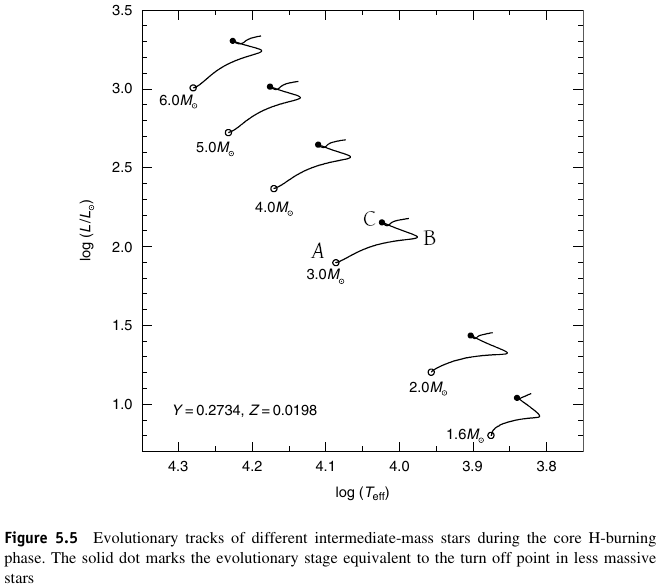
\includegraphics[trim={0cm 0cm 0 0},clip, keepaspectratio,width=0.99\textwidth]{HRD-UMS}\label{fig:HRD-UMS}\end{figure}
\end{column}\begin{column}{0.5\textwidth}
Higher T: CNO dominant: $\epsilon_{CNO}$ steeper:convective core (\xaumenta{M^*}, \xaumenta{M_{con}}, \xaumenta{P_{rad}}, \xdiminuisce{\nad{}}.
\end{column}\end{columns}
\end{frame}

\begin{frame}{Overall contraction and Overshooting ($M>10\msun{}$)}
\begin{columns}[T]\begin{column}{0.5\textwidth}
\begin{figure}[!ht]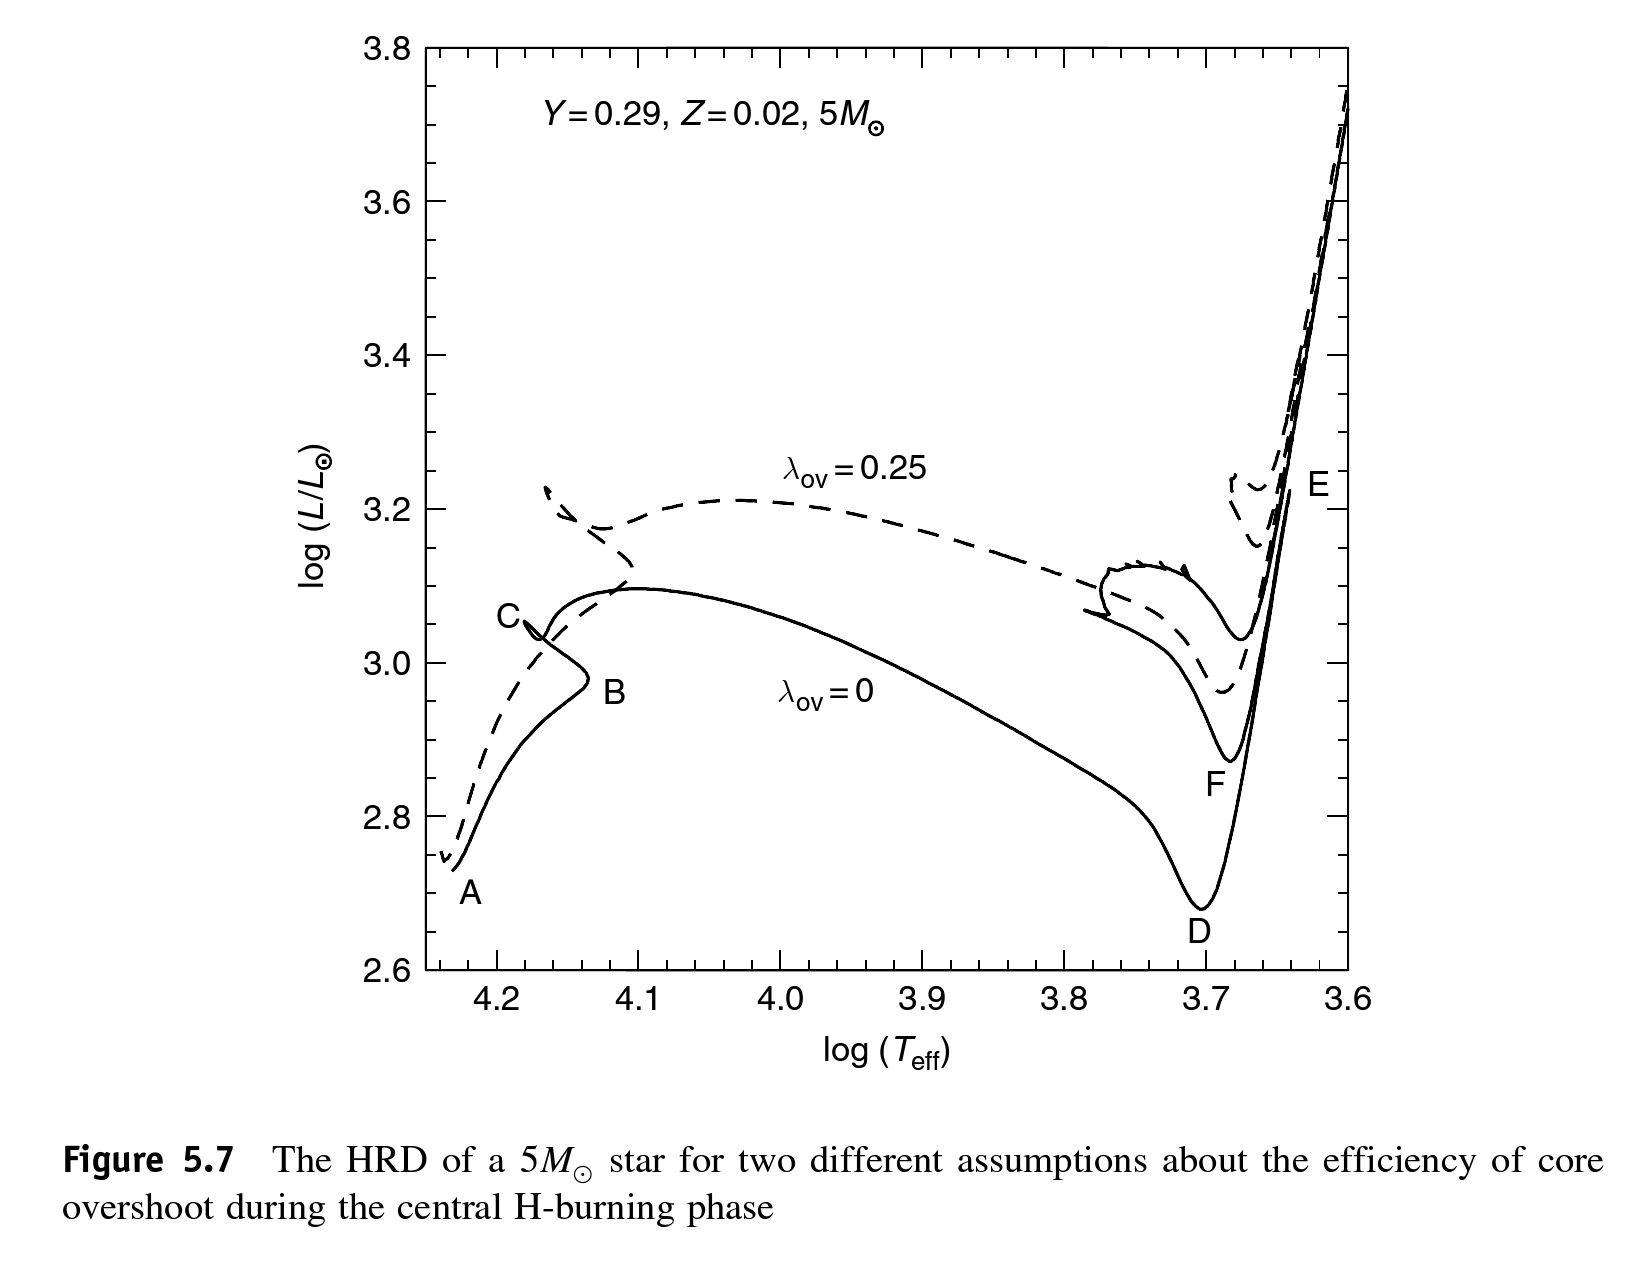
\includegraphics[trim={0cm 0cm 0 0},clip, keepaspectratio,width=0.99\textwidth]{HRD-overshoot}\label{fig:HRD-overshoot}
\end{figure}
\end{column}
\begin{column}{0.5\textwidth}
\begin{block}{What increases convective core}
\begin{itemize}
\item Changes in physical input
\item Stellar rotation
\item Physical overshooting
\end{itemize}
\end{block}
\begin{block}{Overall contraction}

\end{block}
\end{column}\end{columns}
\begin{block}{Effects of increased convective core}
\begin{itemize}
\item \xaumenta{M_c}, \xaumenta{\mu} (involve more mass), \xaumenta{L}
\item Longer central H-burning
\item Larger He core at end of MS: brighter He-burning phase star, shorted lifetime
\end{itemize}
\end{block}
\begin{block}{\sch vs Ledoux in-stability criterion}
In radiative region the retracting convective core leave chem composition gradient; but \xaumenta{He}, \xdiminuisce{\kappa}
\end{block}
\end{frame}

\subsection{Easurimento H centrale}

\begin{frame}{Esaurimento H per stelle di S superiore/inferiore}

\end{frame}

\subsection{Combustione He}

\begin{frame}{Fase subgigante rossa (SGB): H-burning shell}
Turnoff; overall contraction;Gap di hertzsprung;
\end{frame}

\begin{frame}{Fase di gigante rossa (innesco He)}
primo dredge-up; RGB transition mass; morfologia RGB per stelle piccola/intermedia;
Dipendenza RGB-transition mass da composizione;
Massa del core di elio all'innesco in funzione della massa stellare
Luminosit\'a tip rgb vs massa, massa nucleo He a innesco, composizione
bump rgb;
Innesco He a flash per piccole masse
\end{frame}

\begin{frame}{Dipendenza da He/composizione iniziale del SG-RG branch}

\end{frame}

\begin{frame}{Evoluzione da ZAHB}
combustion di He per stelle medio-grandi; clump He; loop He; Esaurimento He centrale: autotrascinamento del nucleo, semiconvezione e pulsi convettivi
\end{frame}

\begin{frame}{Discussioni parametri che influenzano HB}
Parametro R per determinazione He
\end{frame}

\subsection{Ramo asintotico (AGB)}

\begin{frame}{Evoluzione in AGB}
Ingresso in agb: clump. AGB manqu\'e. Secondo Dredge-up; pulsi termici; terzo dredge-up
\end{frame}

\begin{frame}{Nucleosintesi in AGB}
Elementi s:tasca C13. Produzione di Li
\end{frame}

\subsection{Destino finale di stelle massicce}

\begin{frame}{Destino finale di stelle di varia massa}
nane bianche di He, C/O, O/Ne; supernovae di tipo II da deflagrazione del carbonio e cattura elettronica su nuclei; supernovae di tipo II da fotodisintegrazione del ferro; Caratteristiche di pre-SN; Neutronizzazione esplosiva e esplosione ritardata; classificazione SN in base a spettro e morfologia curva di luce
\end{frame}

\begin{frame}{Caratterizzazione SNII}
$Fe60$ come indicatore esplosioni nelle vicinanze della terra negli ultimi milioni di anni; Interazione neutrini-nucleo denso: intrappolamento e tempi scala emissione; stima energia emessa: neutrini, fotoni, fronte di shock; SN1987A: flusso di neutrini e osservazione in bande EM
\end{frame}


\begin{frame}{Evoluzione di nane bianche}

\end{frame}

\subsection{Modello Solare standar}

\begin{frame}{Caratteristiche e metodo di calcolo}
eliosismologia e neutrini
\end{frame}

\subsection{Stelle pulsanti}

\begin{frame}{Striscia di instabilit\'a e tipi di stelle pulsanti}
RR LyrAE: diagramma di Bailey, curve di luce; relazioni periodo-luminosit\'a, massa-temperatura effettiva.
Parametro A come indicatore di He.
Stelle cefeidi; dicotomia di Oosterhoff
\end{frame}